\documentclass[conference]{IEEEtran}
\IEEEoverridecommandlockouts
% The preceding line is only needed to identify funding in the first footnote. If that is unneeded, please comment it out.

\usepackage{cite}
\usepackage{amsmath,amssymb,amsfonts}
\usepackage{algorithmic}
\usepackage{graphicx}
\usepackage{textcomp}
\usepackage{xcolor}
\def\BibTeX{{\rm B\kern-.05em{\sc i\kern-.025em b}\kern-.08em
    T\kern-.1667em\lower.7ex\hbox{E}\kern-.125emX}}
\begin{document}

\title{Klasifikasi Kemenangan pada Dataset Game League of Legends dengan Metode Decision Tree\\
{\footnotesize \textsuperscript{*}Note: Sub-titles are not captured in Xplore and
should not be used}
\thanks{Identify applicable funding agency here. If none, delete this.}
}

\author{\IEEEauthorblockN{1\textsuperscript{st} Meynabel Dimas Wisodewo}
\IEEEauthorblockA{\textit{Teknik Informatika} \\
\textit{Universitas Negeri Malang}\\
Malang, Indonesia \\
dwisodewo@gmail.com}
\and
\IEEEauthorblockN{2\textsuperscript{nd} Yuveta Rosabella}
\IEEEauthorblockA{\textit{Teknik Informatika} \\
\textit{Universitas Negeri Malang}\\
Malang, Indonesia \\
yuvetarosabela@gmail.com}
}

\maketitle

\begin{abstract}
mem-break down 0.85
\end{abstract}

\begin{IEEEkeywords}
Decision Tree, Classification, League of Legends, Game
\end{IEEEkeywords}

\section{Latar Belakang}
League of Legends (disingkat LoL) adalah video game arena pertempuran online multi-pemain yang dikembangkan dan diterbitkan oleh Riot Games untuk Microsoft Windows dan macOS.  Game ini mengikuti model freemium dan didukung oleh transaksi mikro, dan terinspirasi oleh Warcraft III: mod Frozen Throne, Defense of the Ancients. 

Di League of Legends, pemain berperan sebagai "summoner" yang tak terlihat yang mengontrol "juara" dengan kemampuan unik dan bertempur melawan tim pemain lain atau juara yang dikendalikan komputer.  Tujuannya biasanya untuk menghancurkan "Nexus" tim lawan, sebuah struktur yang terletak di jantung pangkalan yang dilindungi oleh struktur pertahanan, meskipun ada mode permainan lain yang berbeda.  Setiap pertandingan League of Legends berbeda, dengan semua juara memulai dengan cukup lemah tetapi bertambah kuat dengan mengumpulkan item dan pengalaman selama pertandingan. Para juara dan latar memadukan berbagai elemen, termasuk fantasi tinggi, steampunk, dan horor Lovecraftian.

League of Legends adalah game 3D, arena pertempuran online multiplayer orang ketiga. Game ini terdiri dari tiga mode game yang sedang berjalan: Summoner's Rift, Twisted Treeline, dan Howling Abyss. Mode game lain, The Crystal Scar, telah dihapus. Pemain berlaga dalam pertandingan, rata-rata berlangsung antara 20 hingga 60 menit.  Dalam setiap mode permainan, tim bekerja sama untuk mencapai kondisi kemenangan, biasanya menghancurkan bangunan inti (disebut Nexus) di pangkalan tim musuh setelah melewati garis struktur pertahanan yang disebut menara, atau menara.

Dalam semua mode permainan, pemain mengontrol karakter yang disebut juara, dipilih atau ditugaskan setiap pertandingan, yang masing-masing memiliki serangkaian kemampuan unik. Champions memulai setiap pertandingan di level rendah, dan kemudian mendapatkan pengalaman selama pertandingan untuk mencapai level maksimum 18. Mendapatkan level juara dalam pertandingan memungkinkan pemain untuk membuka kemampuan khusus juara mereka dan menambah mereka dalam sejumlah cara unik untuk  setiap karakter.  Jika seorang juara kehilangan kesehatannya, mereka dikalahkan tetapi secara otomatis dihidupkan kembali di markas mereka setelah melewati waktu yang cukup.  Pemain juga memulai setiap pertandingan dengan jumlah emas yang rendah, dan bisa mendapatkan emas tambahan sepanjang pertandingan dengan berbagai cara: dengan membunuh karakter non-pemain yang dikenal sebagai antek dan monster;  dengan membunuh atau membantu membunuh pemain musuh;  dengan menghancurkan struktur musuh;  secara pasif dari waktu ke waktu;  dan melalui interaksi item yang unik atau kemampuan juara.  Emas ini kemudian dapat dihabiskan sepanjang pertandingan untuk membeli item dalam game yang semakin menambah kemampuan dan gameplay masing-masing juara dalam berbagai cara.  Pengalaman juara, emas yang didapat, dan barang yang dibeli spesifik untuk setiap pertandingan dan tidak terbawa ke pertandingan berikutnya.  Dengan demikian, semua pemain memulai setiap pertandingan dengan pijakan yang relatif sama dengan tim lawan mereka.

Decision tree adalah salah satu metode klasifikasi yang paling populer, karena mudah untuk diinterpretasi oleh manusia. Decision tree adalah model prediksi menggunakan struktur pohon atau struktur berhirarki. Konsep dari pohon keputusan adalah mengubah data menjadi decision tree dan aturan-aturan keputusan. Manfaat utama dari penggunaan decision tree adalah kemampuannya untuk mem-break down proses pengambilan keputusan yang kompleks menjadi lebih simple, sehingga pengambil keputusan akan lebih menginterpretasikan solusi dari permasalahan.

Pada beberapa kasus pemain kesusahan dalam memenangkan lomba ini. Misal pemain tidak mahir dalam menggunakan karakter yang di pakai dan pemilihan item yang salah pada karakter yang digunakan. Dari kasus tersebut dapat dibuat permasalahan pada paper ini yaitu untuk klasifikasi menang kalah pada game League Of Legends menggunakan metode Decision Tree.

\section{Kajian Pustaka}
\subsection{Dataset League of Legends}
Dataset adalah objek yang merepresentasikan data dan relasinya di memory. Strukturnya mirip dengan data di database. Dataset berisi koleksi dari datatable dan datarelation. League of Legends adalah game 3D, arena pertempuran online multiplayer orang ketiga. Game ini terdiri dari tiga mode game yang sedang berjalan: Summoner’s Rift, Twisted Treeline, dan Howling Abyss. Mode game lain, The Crystal Scar, telah dihapus. Pemain berlaga dalam pertandingan, ratarata berlangsung antara 20 hingga 60 menit. Dalam setiap mode permainan, tim bekerja sama untuk mencapai kondisi kemenangan, biasanya menghancurkan bangunan inti (disebut Nexus) di pangkalan tim musuh setelah melewati garis struktur pertahanan yang disebut menara, atau menara.

\subsection{Preprocessing}
Preprocessing merupakan tahapan awal dalam mengolah data input sebelum memasuki proses tahapan utama dari metode Latent Semantic Analysis (LSA). Preprocessing text dilakukan untuk tujuan penyeragaman dan kemudahan pembacaan serta proses LSA selanjutnya (Aji P., Baizal SSi. and Firdaus S.T., 2011)

\subsection{K-Fold Cross Validation}
Membuat model untuk “Machine Learning” bisa sangat sulit.  Biasanya, kami membagi set data menjadi set pelatihan dan pengujian dan menggunakan set pelatihan untuk melatih model dan set pengujian untuk menguji model.  Kami kemudian mengevaluasi kinerja model berdasarkan metrik kesalahan untuk menentukan akurasi model.  Namun metode ini, tidak terlalu dapat diandalkan karena akurasi yang diperoleh untuk satu set tes bisa sangat berbeda dengan akurasi yang diperoleh untuk set tes yang berbeda.  K-fold Cross Validation (CV) memberikan solusi untuk masalah ini dengan membagi data menjadi lipatan dan memastikan bahwa masing-masing lipatan digunakan sebagai set pengujian di beberapa titik.  Artikel ini akan menjelaskan secara sederhana apa itu K-Fold CV dan bagaimana menggunakan pustaka sklearn untuk melakukan K-Fold CV.

K-Fold CV adalah tempat kumpulan data yang diberikan dibagi menjadi sejumlah K bagian / lipatan di mana setiap lipatan digunakan sebagai set pengujian di beberapa titik.  Mari kita ambil skenario validasi silang 5-Lipat (K = 5).  Di sini, kumpulan data dibagi menjadi 5 lipatan.  Pada iterasi pertama, lipatan pertama digunakan untuk menguji model dan sisanya digunakan untuk melatih model.  Pada iterasi kedua, lipatan kedua digunakan sebagai set pengujian sementara sisanya berfungsi sebagai set pelatihan.  Proses ini diulangi sampai setiap lipatan dari 5 lipatan telah digunakan sebagai set pengujian.

\subsection{Decision Tree}
Decision tree adalah salah satu metode klasifikasi yang paling populer, karena mudah untuk diinterpretasi oleh manusia. Decision tree adalah model prediksi menggunakan struktur pohon atau struktur berhirarki. Konsep dari pohon keputusan adalah mengubah data menjadi decision tree dan aturan-aturan keputusan. Manfaat utama dari penggunaan decision tree adalah kemampuannya untuk mem-break down proses pengambilan keputusan yang kompleks menjadi lebih simple, sehingga pengambil keputusan akan lebih menginterpretasikan solusi dari permasalahan.

Decision Tree Ini adalah bagan aliran seperti struktur pohon, di mana setiap node internal menunjukkan tes pada atribut, setiap cabang menunjukkan hasil tes, dan setiap node daun memegang label kelas.  Node paling atas dalam pohon adalah simpul akar [1].  Diberikan tuple, X, yang label kelas terkait tidak diketahui, nilai atribut tuple diuji terhadap pohon keputusan.  Jalur dilacak dari akar ke simpul daun, yang menampung prediksi kelas untuk tupel itu. Decision tree berguna karena konstruksi classifier pohon keputusan tidak memerlukan pengetahuan domain apa pun.  Itu dapat menangani data hidimensional.  Langkah-langkah pembelajaran dan klasifikasi induksi pohon keputusan sederhana dan cepat.  Representasi pengetahuan yang mereka peroleh dalam bentuk pohon mudah diasimilasi oleh pengguna.  Pengklasifikasi pohon keputusan memiliki akurasi yang baik [2].
Decision Tree mencoba menemukan partisi optimal dari ruang pengamatan yang mungkin, terutama dengan cara pemisahan rekursif berikutnya.

\section{Metodologi}
\subsection{Objek Penelitian}
Objek yang diteliti dalam penelitian ini adalah mengamati statistik dari game league of legends. Dalam penelitian ini dilakukan pertandingan beberapa kali dan atribut-atribut menangnya diambil sata statistiknya.

\subsection{Pengumpulan Data}
Merupakan salah satu teknik pengambilan keputusan kriteria majemuk yang digunakan untuk melakukan analisis dalam penelitian keputusan terbaik dari sejumlah alternatif dengan tujuan menghasilkan perolehan yang optimal.
Pada tahap ini dilakukan untuk pengumpulan data dan informasi secara lengkap dan akurat. Data yang sudah diperoleh akan di training pada proses selanjutnya. Berikut adalah tahapan metode pengumpulan data antara lain :
1 pengelompokan kriteria menang dan kalah 
Kegiatan ini dilakukan dengan tujuan untuk mendapatkan parameter yang digunakan untuk memprediksi kemenangan.
2. Mengambil data nilai kemampuan karakter
Kegiatan ini bertujuan untuk mendapatkan nilai dari setiap karakter yang sudah didapatkan sebelumnya.

\subsection{Unsur Penilaian}
Setelah dilakukan pengumpulan data maka selanjutnya diperoleh beberapa kriteria karakter yang akan digunakan sebagai paramater. Kriteria tersebut antara lain :
\begin{itemize}
\item jumlah kills dari karakter baron, dragon
\item nilai first kills dari karakter baron, dragon
\item nilai first kills, first tower, towerkills
\end{itemize}

\subsection{Rencana Penelitian}
Dalam perancangan sistem dengan menggunakan metode Decision Tree, dibutuhkan proses yang dapat dapat menghasilkan output dari sistem keputusan, oleh karena itu dibuatlah blok diagram yang fungsinya untuk menggambarkan sistem secara garis besar. Berikut adalah alur penelitian. 
Input masing-masing parameter -> sistem klasifikasi decision tree -> output hasil klasifikasi menang kalah

\subsection{Preprocessing}
Feature Selection adalah suatu kegiatan pemodelan atau penganalisaan data yang umumnya dapat dilakukan secara preprocessing dan bertujuan untuk memilih fitur yang berpengaruh (fitur optimal) dan mengesampingkan fitur yang tidak berpengaruh, (Rehat, 2009). Feature Selection atau Feature Reduction adalah suatu kegiatan yang umumnya bisa dilakukan secara preprocessing dan bertujuan untuk memilih feature yang berpengaruh dan mengesampingkan feature yang tidak berpengaruh dalam suatu kegiatan pemodelan atau penganalisaan data. Ada banyak alternatif yang bisa digunakan dan harus dicoba-coba untuk mencari yang cocok. Secara garis besar ada dua kelompok besar dalam pelaksanaan feature selection: Ranking Selection dan Subset Selection.

himpunan fitur yang tersedia untuk meningkatkan aplikasi dari suatu algoritma pembelajaran. Feature Selection digunakan dibanyak area aplikasi sebagai alat untuk menghilangkan fitur yang tidak relevan dan atau fitur berlebihan. Sebuah fitur dikatakan tidak relevan jika memberikan sedikit informasi, sedangkan sebuah fitur dikatakan berlebihan jika informasi yang diberikan adalah informasi yang terkandung dalam fitur lain (tidak memberikan informasi baru).
Ada empat langkah yang dilakukan dalam feature selection (Dash, 1997) yaitu:

\begin{itemize}
\item Prosedur generasi (pembangkitan), untuk menghasilkan calon subhimpunan berikutnya dapat dilakukan dengan beberapa cara yaitu : lengkap, heuristik dan acak.
\item Evaluasi fungsi, untuk mengevaluasi subhimpunan, dengan cara mengukur jarak, informasi, konsistensi, ketergantungan, dan mengukur tingkat kesalahan klasifikasi.
\item Kriteria penghentian, untuk memutuskan kapan harus berhenti, dengan cara melihat nilai ambang batas (threshold), diawali dengan sejumlah pengulangan dan sebuah ukuran subhimpunan fitur terbaik.
\item Prosedur validasi, untuk memeriksa apakah subhimpunan valid. (opsional).
\end{itemize}

\subsection{Decision Tree}

Decision Tree Ini adalah bagan aliran seperti struktur pohon, di mana setiap node internal menunjukkan tes pada atribut, setiap cabang menunjukkan hasil tes, dan setiap node daun memegang label kelas.  Node paling atas dalam pohon adalah simpul akar [1].  Diberikan tuple, X, yang label kelas terkait tidak diketahui, nilai atribut tuple diuji terhadap pohon keputusan.  Jalur dilacak dari akar ke simpul daun, yang menampung prediksi kelas untuk tupel itu. Decision tree berguna karena konstruksi classifier pohon keputusan tidak memerlukan pengetahuan domain apa pun.  Itu dapat menangani data hidimensional.  Langkah-langkah pembelajaran dan klasifikasi induksi pohon keputusan sederhana dan cepat.  Representasi pengetahuan yang mereka peroleh dalam bentuk pohon mudah diasimilasi oleh pengguna.  Pengklasifikasi pohon keputusan memiliki akurasi yang baik [2]. Decision Tree mencoba menemukan partisi optimal dari ruang pengamatan yang mungkin, terutama dengan cara pemisahan rekursif berikutnya.

Algoritma decision tree adalah algoritma induksi top-down.  Tujuan dari algoritma ini adalah untuk membangun pohon yang memiliki daun yang homogen mungkin.  Langkah utama dari algoritma ini adalah untuk terus membagi daun yang tidak homogen menjadi daun yang homogen mungkin.

\section{Analisis}
Import Data menggunakan library pandas. Dataset memiliki feature berjumlah 65. Tentu saja feature sebanyak ini tidak akan digunakan semuanya. Maka dari itu dataset akan dilakukan preprocessing terlebih dahulu.

Setelah memilah feature secara manual, selanjutnya memilah berdasarkan Missing Value Ratio. Disini kami hanya akan menggunakan feature dengan missing value berjumlah dibawah 20\%. Untungnya data yang kami gunakan tidak memiliki missing value, sehingga jumlah feature tetap sama.

Kemudian memilah feature berdasarkan Low Variance Filter. Feature dengan variance data kurang dari 10\% tidak akan digunakan. Setelah dipilah berdasarkan low variance filter, feature berkurang menjadi 33.

Setelah itu dilakukan preprocessing yang terakhir dengan menggunakan Random Forest. Dengan menggunakan Random Forest, akan diketahui urutan feature terbaik sehingga dapat kita pilih beberapa feature yang terbaik. Dalam kasus ini, kita akan menggunakan 15 feature terbaik. Tingkat kedalaman maksimum kami tentukan sejumlah 5, karena nantinya kami akan melakukan klasifikasi dengan decision tree dengan kedalaman maksimum 5. Criterion kami set entropy untuk menentukan susunan tree berdasarkan information gain. Tingkat kepentingan feature akan ditampilkan dalam bentuk grafik.

Setelah diketahui urutan feature dari yang paling penting, selanjutnya menghilangkan feature yang tidak masuk dalam peringkat 15 feature terbaik yang telah diketahui dengan metode Random Forest. Setelah itu saatnya melakukan klasifikasi dengan metode Decision Tree karena data sudah siap untuk digunakan. Criterion pada model diset entropy untuk menentukan susunan tree berdasarkan information gain. Criterion yang digunakan harus sama dengan yang digunakan dalam preprocessing menggunakan random forest, begitu juga dengan maksimal kedalaman pada tree.

Setelah selesai melakukan klasifikasi pada data tes, selanjutnya adalah melakukan evaluasi untuk mengetahui tingkat keakuratan model yang telah dibuat. Evaluasi dilakukan dengan menghitung akurasi, presisi, dan recall.

\begin{figure}
\caption{Peringkat Feature terbaik menggunakan Random Forest}
\begin{center}
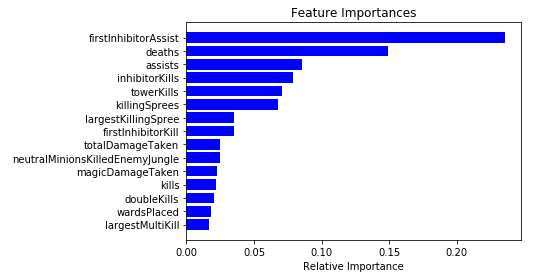
\includegraphics[scale=.6]{FeatureImportances.png}
\end{center}
\end{figure}

Setelah melakukan beberapa tahap preprocessing dan data sudah siap untuk digunakan, saatnya memisahkan data untuk training dengan data untuk testing. Kami membagi data untuk training dan testing sama rata agar model tidak mengalami overfitting. Kemudian mempersiapkan model untuk klasifikasi dengan Decision Tree dan melakukan traiining dengan data yang telah dibagi sebagai data training. Kedalaman maksimal untuk tree kami set sejumlah 5, karena tree yang terlalu dalam akan menyebabkan overfitting pada model. Criterion kami set ke entropy untuk menentukan susunan tree berdasarkan information gain.

Setelah model dilakukan training, saatnya melakukan klasifikasi dengan data yang telah dibagi sebagai data testing. Kemudian melakukan evaluasi untuk melihat berapa tingkat keakuratan model yang telah dibuat. Evaluasi dilakukan dengan menghitung nilai akurasi, presisi dan recall.

\begin{figure}
\caption{Susunan Tree berdasarkan Information Gain}
\begin{center}
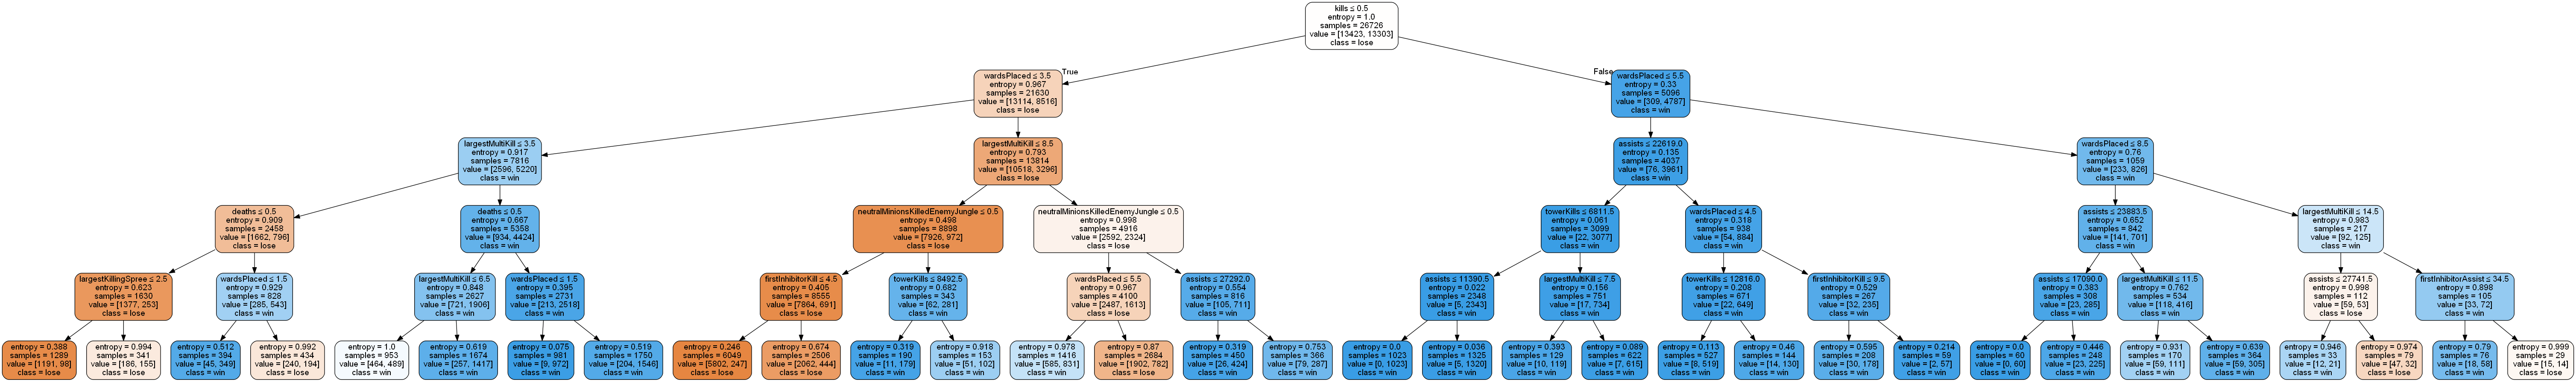
\includegraphics[scale=.04]{DecisionTree.png}
\end{center}
\end{figure}

\begin{figure}
\caption{Hasil Evaluasi)}
\begin{center}
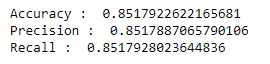
\includegraphics[scale=1]{Evaluasi.png}
\end{center}
\end{figure}

\section*{Kesimpulan}
Dataset League of Legends ini dilakukan klasifikasi dengan metode Decision Tree dan memiliki nilai akurasi sebesar 0.8517922622165681, nilai presisi sebesar 0.8517887065790106 dan nilai recall sebesar 0.8517928023644836. Dapat dilihat bahwa hasil evaluasi menunjukkan nilai yang cukup tinggi. Ini berarti hasil klasifikasi model cukup akurat.

\begin{thebibliography}{00}
\bibitem{b1}  Xindong Wu, Vipin Kumar, J. Ross Quinlan, Joydeep Ghosh, Qiang Yang, Hiroshi Motoda, Geoffrey J. McLachlan, Angus Ng, Bing Liu and Philip S. Yu, et al., "Top 10 algorithms in data mining", Knowledge and Information Systems, Vol. 14, No. 1, 1-37, DOI: 10.1007/s10115-007- 0114-2.
\bibitem{b2} Hang Yang, Fong, S, "Optimized very fast decision tree with balanced classification accuracy and compact tree size," Data Mining and Intelligent Information Technology Applications (ICMiA), 2011 3rd International Conference on, Pp.57-64, 24-26 Oct. 2011.
\bibitem{b3} Lee, Michael. (2010). Perancangan Klasifikasi Penerimaan Beasiswa Menggunakan Algoritma ID3 (Iterative Dichtomizer Three). Salatiga: FTI UKSW.
\bibitem{b4} Florin Gorunescu. 2011.Data Mining: Concept, Model and Techniques. Berlin :Springer
\bibitem{b5} Fadlan Amirudin, Eneng Tita Tosida, Irma Anggraeni. (n.d.). Implementasi Algoritma Classification and Regression Tree (CART) untuk Klasifikasi Bantuan Usaha Mikro Kecil Menengah (UMKM) Jasa Telematika Indonesia.
\bibitem{b6} Bhargavi, S. Jyothi. (2009). Applying Naive Bayes Data Mining Techniques for Classification of Agricultural Land Soils. International Journal of Computer Science and Network Security Vol.9, No.8, 117-122.
\bibitem{b7} Mardi, Y. (n.d.). Data Mining: Klasifikasi Menggunakan Algoritma C4.5. Jurnal Endik Informatika Vol.2, No.2, 213-219.
\bibitem{b8} Fadlan Amirudin, Eneng Tita Tosida, Irma Anggraeni. (n.d.). Implementasi Algoritma Classification and Regression Tree (CART) untuk Klasifikasi Bantuan Usaha Mikro Kecil Menengah (UMKM) Jasa Telematika Indonesia.
\bibitem{b9} Rani, L. N. (2015). Klasifikasi Nasabah Menggunakan Algoritma C4.5 sebagai Dasar Pemberian Kredit. Jurnal KomTekInfo Vol. 2, No. 2, 33-38.
\bibitem{b10} Nafiiyah, N. (2015). Algoritma CART dalam Penentuan Pohon Keputusan Sertifikasi Guru. Jurnal SPIRIT Vol.7, No.2
\end{thebibliography}
\vspace{12pt}
\end{document}
